\documentclass[onecolumn,preprintnumbers,amsmath,amssymb]{revtex4}
\newcommand{\gguide}{{\it Negative Correlation in Traffic Recovery}}
%Uncomment next line if AMS fonts required
\usepackage[dvips]{graphicx}% Include figure files
\usepackage{dcolumn}% Align table columns on decimal point
\usepackage{float}
\usepackage{bm}% bold math
\usepackage{color}


%\nofiles

\begin{document}

\title{Negative Correlation in Traffic Recovery}

\author{Yichao Zhang$^{1}$}
\email{yiczhang@cs.ucl.ac.uk}

\author{Xing Li$^{1}$}
\email{15000218895@163.com}


\author{Jihong Guan$^{1}$}
\email{jhguan@tongji.edu.cn}


\author{Shuigeng Zhou$^{2}$}
\email{sgzhou@fudan.edu.cn}

\affiliation{$^{1}$Department of Computer Science and Technology, Tongji University, 4800 Cao'an Road, Shanghai 201804, China}

\affiliation{$^{2}$Department of Computer Science and Engineering, Fudan University, Shanghai 200433, China \\ Shanghai Key Lab of Intelligent Information Processing, Fudan University, Shanghai 200433, China}

\begin{abstract}
With the rapid development of information and communication technology, we can access a wide range of network data. These data sets offer us the opportunity to analyze and predict network revolution. In this paper, we have proposed a way which combines link prediction methods to solve the traffic congestion problem. Based on the congested traffic line, we will predict the likelihood of new routes. One different from the link prediction problem is that in the traditional link prediction our goal was to find the edges to be created in the future, while in our traffic problem we have already known the edges to be predicted, our goal was to predict the sequence of these edges. Besides the algorithms we have proposed, we have conducted varies experiments to prove our methods to be effective to reduce the congestion index of the traffic. This work is an exploration of using link prediction method in the traffic problem, it provides a new view in the traffic control problem and may further affect the link prediction usage in the traffic field. 
\end{abstract}

\pacs{87.23.Ge, % Negative Correlation
02.50.Le,       % Traffic Recovery
89.75.Fb        % Link Prediction
}

\maketitle

\section*{INTRODUCTION\protect}

Since 1736 Euler defined and solved the Seven Bridges problem of Königsberg, there was not much ground breaking development in the complex network research area until 1960s, when the Erdos-Renyi random graph model (ER–model) was introduced. A new wave of research was set off by Watts and Strogatz who published a paper about the small– world effect in 1998 and introduction of the scale–free network model by Barabasi and Albert one year later. The number of publications in the last 17 years in complex networks is more than the total appearance before 1999. In our living world, many systems can be modeled as complex networks where nodes represent the basic units of a system and links stands for the interactions between the nodes\cite{TFWN}. Complex networks has been a research field focus on not only science but also engineering for the last few decades\cite{PSV,AEM,KIG,BTS,LZYC,HHM,RAA,SND,MEJ,SBV}.


Modern world depends greatly on the efficient operation of many critical infrastructures such as Internet, airlines, power grid and so on\cite{TCIC}. Researcheres on such fields realize that such systems can be modeled within the framework of complex networks. Traffic on such networks is a vital problem. Recently, more attentions has been given to the traffic congestion problem in transportation networks, understanding network congestion has become a subject of intense research in this field. 

Zhao et al. proposed two models to address the problem: (1) The capacity of delivery of each node is proportional to its degree; (2) The delivery capacity of each node is proportional to its betweenness. They have found that in the first model, random networks and scale-free networks are more tolerant to congestion than regular networks
and Cayley trees. For the second model, the crowded degree is independent of the network topology and size, so this model may be useful for communication protocols\cite{LZY}.
In their work, Boccaketti et al. thought that in transportation networks, the factors that affect the global performance are the traffic load of a road, that is to say the number of the passengers in the airport or the passengers in the subways. They also doing experiments to remove a small fraction of nodes simulating the breakdown of an Internet router or transportation system, such removals will change the shortest paths between nodes and the distribution of the loads and creating overloads on some nodes.
After the experiment, they found that homogeneous network does not experience cascading failures due either to random breakdown or to intentional attacks. While for the heterogeneous network, cascades triggered by the attack on a key node can causes serious congestion problem, homogeneous networks appear to be more resistant to cascading failures than the heterogeneous ones\cite{SBV}.
Toroczkai et al. have compared the congestion in gradient networks generated by either random or scale-free substrates, finding that in the latter case the networks are less prone to jamming\cite{ZTKE,ZTBE}.
Roger et al. thought that the system only behaves efficiently when the amount of packages handled is small enough. The network collapses above a certain threshold and some packages is accumulated. They found that independently of the topology(1D, 2D and Cayley), the collection of models can be split into three groups according to how the network collapses. In the first group, agents deliver more packets as they are more congested, although their capability decreases, and the network never collapses. In the second group, agents deliver always the same number of packets independently of their load—number of packets to deliver; this behavior leads to a continuous phase transition. Finally, when agents deliver fewer packets as their loads increase, the transition to the congested phase is discontinuous and the network collapses in an inhomogeneous way giving rise to congestion nuclei\cite{RGA}.%comes originally from the paper


Compared with the potential costs of changing the structure of well-established networked systems, proposals of clever routing criteria seem to be more practical
and thus attract much interest.
Daniele et al. tested a trade-off strategy between traffic based and topological based
routing on scale-free networks and found that traffic control is useless in homogeneous networks but may useful in inhomogeneous networks\cite{DDL}. 
Gang Yan et al. propose a routing strategy to improve the transportation efficiency on complex networks. Instead of using the routing strategy for shortest path, they give a generalized routing algorithm to find the so-called "efficient path", which considers the possible congestion in the nodes along actual paths. Since the nodes with the
largest degree are very susceptible to traffic congestion, an effective way to improve traffic and control congestion can be redistributing traffic load in central nodes to other non-central nodes. Simulation results indicate that the network capability in processing traffic is improved more than 10 times by optimizing the efficient path\cite{GYT}.
Xiang et al. propose a global dynamic routing strategy for network systems based on the information of the queue length of nodes. Under this routing strategy, the traffic
capacity is further improved compared with Gang\cite{GYT}. With time delay of updating node queue lengths and the corresponding paths, the system capacity remains constant, while the travel time for packets increases\cite{XLM}.
Danila et al.'s algorithm balances traffic on a network by minimizing the maximum node betweenness with as little path lengthening as possible, thus being useful in cases when networks are jamming due to queuing overload. By using the resulting routing table, a network can sustain significantly higher traffic without jamming than in the case of traditional shortest path routing\cite{BDY}.
Tan Fei et al. proposed a routing algorithm that combines static structural properties and dynamic traffic conditions together and therefore can balance the traffic between hubs and peripheral nodes more effectively\cite{FTY}.
Guan et al. focus their research on traffic dynamics of a spatial scale-free network with the restriction of bandwidth proportional to link Euclidean distance, and a new routing strategy is proposed with consideration of both Euclidean distance and betweenness centralities (BC) of edges. It is found that compared with the shortest distance path (SDP) strategy and the minimum betweenness centralities (MBC) of links strategy, their strategy under some parameters can efficiently balance the traffic load and avoid excessive traveling distance which can improve the spatial network capacity and some system behaviors reflecting transportation efficiency, such as average packets traveling time, average packets waiting time and system throughput, traffic load and so on\cite{XLMD}.



In practice it is often difficult to change a network’s routing protocol or topology. The above works have assumed that all nodes or links are assigned with uniform
resources. This simplified scenario allows researchers to study the pure contribution of the routing algorithms and the topology. However it is unrealistic as in real networks resources are rarely distributed uniformly.
Zhang et al. come up with a practical and effective approach to allocate the resources in a network such that network elements that handle higher volumes of traffic load have more resources whereas those that handle less load have fewer resources. The results show that our scheme enhances the transmission capacity of networks with heterogeneous structures by up to two orders of magnitude\cite{GQZ}.

Link prediction in complex network is one of the popular research topics. Generally, the prediction problem is mainly studied from two angles: (i) network structure and (ii) attributes of nodes and connections. Structure reflects the information about network topology. Majority of the progress in the area of structure based prediction has been made by mathematicians and physicists. Some of the well known structure based prediction methods are Common Neighbor, Preferential Attachment Index, Adamic-Adar Index, Katz, etc. The link prediction problem also has been studied from the angle of the network attribute information. The majority of attribute-based prediction methods follow a machine learning approach, i.e. they use classification–based methods to make predictions. Authors \cite{LPU,NPA,LPC,WWC,SRM} report that the performance of link prediction improves when machine learning approaches are used. However, this is done using additional network information that is not always available. Since the attribute of nodes is hard to achieve ,so in our research we mainly focus on network structure algorithms.





%Network structures have been studied for many years. First research in this area can be traced back to 1736 when Euler defined and solved the Seven Bridges problem of Königsberg\cite{GTC}. There was not much ground breaking development in the complex network research area until 1960s, when the Erdos-Renyi random graph model (ER–model) was introduced. Due to the fact that there was a lack of large real world data, most of the work had been done on the  analysis of phenomena existing in networked structures. During the time when ER–model was introduced, progress has also been made by sociologists in researching real world human relationships . A new wave of research was set off by Watts and Strogatz who published a paper about the small– world effect in 1998 and introduction of the scale–free net- work model by Barabasi and Albert one year later.

%Link prediction in complex network is one of the popular research topics. Generally, the prediction problem is mainly studied from two angles: (i) network structure and (ii) attributes of nodes and connections. Structure reflects the information about network topology. Majority of the progress in the area of structure based prediction has been made by mathematicians and physicists. Some of the well known structure based prediction methods are Common Neighbor, Preferential Attachment Index, Adamic-Adar Index, Katz, etc. The link prediction problem also has been studied from the angle of the network attribute information. The majority of attribute-based prediction methods follow a machine learning approach, i.e. they use classification–based methods to make predictions. Authors \cite{LPU,NPA,LPC,WWC,SRM} report that the performance of link pre- diction improves when machine learning approaches are used. However, this is done using additional network information that is not always available. Since the attribute of nodes is hard to achieve ,so in our research we mainly focus on network structure algorithms.

%The transportation network is one of the three most important networks created by human society (transportation, energy and information). Network analysis is to explore the spatial relationship (structure) characteristics and service  of transportation system. Because it is closely related to people's lives, Multi-disciplines from different perspectives doing researches on transportation problem.
%Geography focuses on analyzing the spatial pattern, temporal and spatial evolution of transportation networks and their relationship with economic and social development\cite{GME,GOT}. Traffic planning is focused on the study of traffic demand or the impact of traffic on the road network, design and planing\cite{UTN}. Operations research tends to analyze transport network and transportation organization optimization, such as TSP problem, transport problems, vehicle path problems.

%With the rapidly development of modern society, the traffic problem has attracted a lot %of attention. Most of the previous study in transportation mainly focus on the design %of the transportation routes, while it can't avoid congestion totally. Once the %transportation system become congested, we need to find a way to solve it. Link %Prediction method have a history of nearly 20 years, it has become a mature subject.
%Link prediction has been applied in the analysis of social networks, biological %networks such as protein-protein interaction networks, metabolic networks and food %webs, personalized recommendation, etc\cite{NHS,TOM,SPR,TZ,SAD,CAA}. Inspired by link %prediction, we ranked the congested traffic routes(BA network, USAir, Road network) and %recover the routes in order. From our result we can see the reverse of link prediction %method can efficiently recovery the congested routes.


\section*{RELATED WORK\protect}
The simplest framework of link prediction methods is the similarity-based algorithm, where each pair of nodes x and y, is assigned a score $s_x$$_y$, which is directly defined as the similarity between x and y. Similarity-based algorithm are classified into three categories: local indices; global indices; quasi-local indices, which do not require global topological information but make use of more information than local indices\cite{SV}. Considered of computation complexity here in our experiment we use two classic algorithm: PA in local indices and LP in quasi-local indices and other transformed algorithms.

(1) Preferential Attachment Index (PA)\cite{WG}. The mechanism of preferential attachment can be used to generate evolving scale-free networks, where the probability that a new link is connected to the node x is proportional to k$_x$. A similar mechanism can also lead to scale-free networks without growth , where at each time step, an old link is removed and a new link is generated. The probability that this new link will connect x and y is proportional to k$_x$ × k$_y$. Motivated by this mechanism, the corresponding similarity index can be defined as
\begin{equation}
\centerline{
$S_x$$_y$=
k$_x$ * k$_y$
}
\end{equation}


(2) Local Path Index (LP)\cite{AC,LI}. Denote by A the adjacency matrix, where A$_x$$_y$ = 1 if x and y are directly connected, and A$_x$$_y$ = 0 otherwise. Obviously, (A$^2$)$_x$$_y$ is the number of common neighbors of nodes x and y, which is also equal to the number of different paths with length 2 connecting x and y. And if x and y are not directly connected , (A$^3$)$_x$$_y$ is equal to the number of different paths with length 3 connecting x and y. The information contained in A$^3$ can be used to break the degeneracy of the states, and thus we define a new measure as

\begin{equation}
\centerline{
$S$=
A$^2$ + $\varepsilon$A$^3$
}
\end{equation}
The score of $S_x$$_y$ correspond to the element is S. And in our experiment we set 
$\varepsilon$= 0.2.


(3) Three order Similarity Index (SA). This algorithm are proposed in this study, the purpose was to magnify the recovery accuracy of the traffic routes. $\Gamma$$^3$(x) means the set of first order neighbor second order neighbor and third order neighbor in all.
\begin{equation}
\centerline{
$S_x$$_y$=
$|$$\Gamma$$^3$(x) $\cap$ $\Gamma$$^3$(y)$|$
}
\end{equation}

\noindent {\bf The followed four algorithm are the transformer of the above three algorithm.}

(4) Reverse Preferential Attachment Index (RPA). simply put the numerator into denominator, which means nodes with less neighbors play a more important role.


\begin{equation}
S_{xy}=\frac{1}{k_x \times k_y}
\end{equation}

(5) Reverse Add Preferential Attachment Index (RAPA). One different from RPA is that at the denominator part we transfer multiply into add.


%$S_x$$_y$=$\frac{1}{k$_x$ * k$_y$}$
\begin{equation}
S_{xy}=\frac{1}{k_x + k_y}
\end{equation}

(6) Reverse Local Path Index (RLP). simply put the numerator into denominator

\begin{equation}
S=\frac{1}{A^2 + \varepsilon A^3}
\end{equation}
The score of $S_x$$_y$ correspond to the element is S. And in our experiment we set 
$\varepsilon$= 0.2.


(7) Reverse Three order Similarity Index (RSA). simply put the numerator into denominator
\begin{equation}
S_{xy}=\frac{1}{ |\Gamma^3(x) \cap \Gamma^3(y)|}
\end{equation}




\section*{DATASETS\protect}
To verify our methods, we have conducted varies experiments on three kinds of networks. The networks are as below:

\noindent {\bf BA network}

we select the Barabasi-Albert (BA)\cite{BA} model to generate the topological network, the degree distribution of which is a power law p(k) $\propto$ $k^{-3.0}$ where p(k) is the ratio of the nodes with degree k to the number of all nodes in the network. The model could represent the heterogeneous node degree of many real-world networks, including the Internet AS level topology, the logical topology of unstructured P2P distributed systems, and so on. In the simulation, we set the mean degree of the network k=4.

\noindent {\bf USAir}

We got USAir data from pajek datasets, The network is extracted from the USAir transportation system. The data contains 332 nodes and 2126 edges. Nodes in the network are individual cities and edges are airlines between these cities. Notice that this is a undirected network which means if you can buy a ticket from city A to city B then you can also buy a ticket from city B to city A. In some degree, USAir is a kind of BA network, some major City like New York and Los Angeles owns more airlines than small cities.

\noindent {\bf California road network}

The dataset was obtained from Stanford dataset. The original data contains 1,965,206 nodes and 2,766,607 edges. Considered the network is too large for link prediction and traffic simulation, so we split out some small part from the California road network. First we randomly choose a node and take it as the center node, then we use Level Traverse method to spread the network out and we can get different size of road network for our needs. For example, if we take nodeId= 100 as the center node, then we select the node 100’s neighbor and append them into the new network, then append the 100’s neighbor’s Neighbor, and the next steps are as before. In California road network, if we choose nodeId= 800120 as the center node and the spread level is 30 we can get a network with 1285 nodes and 1748 edges.

\noindent {\bf The basic topology statistics of the six networks are summarized in Table I.}

\begin{table}[tbp]
\centering  % 表居中
\begin{tabular}{lccccccc}  % {lccc} 表示各列元素对齐方式,left-l,right-r,center-c
\hline  % \hline 在此行下面画一横线
&$|V|$ &$|E|$ &D &C &$<k>$ &$<d>$ &H\\ 
\hline  BA256 &256 &508 &0.016 &0.075 &3.97 &3.49 &2.17 \\  
\hline  BA512 &512 &1020 &0.008 &0.052 &3.98 &3.68 &2.87 \\
\hline  BA1024 &1024 &2044 &0.004 &0.030 &3.99 &4.07 &2.78\\
\hline USAir &332 &2126 &0.039 &0.625 &12.81 &2.74 &3.46\\
\hline Cal Road 10 &121 &156 &0.021 &0.142 &2.58 &9.54 &1.13\\
\hline Cal Road 20 &409 &525 &0.006 &0.101 &2.57 &17.71 &1.17\\
\hline Cal Road 30 &1285 &1750 &0.002 &0.077 &2.72 &23.28 &1.16\\
\hline
\end{tabular}
\caption{statistics of the six networks.}
\end{table}

$|V|$ is the number of vertices and $|E|$ is the number of edges in a given network. D denotes the density of the network which is to calculate $\frac{2|E|}{|V-1|*|V|}$. A node’s clustering coefficient states that, if there are $k_i$ neighbors owned by a vertex $v_i$ and the maximal feasible edges among them could be $k_i*(k_i – 1)/2$, the local clustering coefficient for the vertex $v_i$ is to calculate $C_i$ = \cite{SW}, where $N_i$ stands for the number of neighbors of $v_i$. C denotes the average clustering coefficient. $|k|$ is the average degree of the network. Here, a shortest path is defined as a path connecting two unconnected nodes with least edges and thus the shortest path distance is the number of edges existed within the shortest path. $<d>$ denotes the average shortest path distance of the network. Degree heterogeneity is a statistical property, which quantitatively characterizes the fluctuation of the degree sequence of a network. This property was frequently mentioned, while its explicit definition was not manifested until a recent work\cite{PML}. To be consistent with previous studies, we denote the degree heterogeneity by H. H is defined as $\frac{2|E|}{|V-1|*|V|}$, where $<k>$ denotes the average degree\cite{KD}.



\section*{EXPERIMENT\protect}

In this section we will give our method to improve the transmission efficiency of the  traffic network, show the simulation results, and then discuss them extensively.

\noindent {\bf 1.Method}

$1)$ In order to test our method we should generate traffic- like topological networks. Here we got three kinds of networks, BA network, USAir network and California road network. To simplify the simulation, they are set to be unweighted and undirected.

$2)$ The next step is to simulate the congestion of the traffic net. We think that in the status of congestion the traffic in the route almost Stagnated, so to some degree it equals the route has been broken. So in this process we randomly select a part of the route, and break them up. Notice that we allow the situation that after the break of the network, there are exists individual nodes.

$3)$ Since we have broken links, so we can use link prediction methods to rank the edges of nonsexist, and determine the sequence of recovery links. One different from link prediction is that in link prediction we will rank all the edges of nonsexist while in route recovery we just need to judge the important of broken edges and recover them in order. Here we have eight methods to recover the routes which was mentioned before. 

$4)$To verify the efficiency of different methods based on link prediction, we have conducted package simulation experiments. Several models have been proposed to simulate packet traffic dynamics on complex networks by introducing random generation of packets in each time step and various routing strategies. We here adopt one widely used before.

{\bf In each time step}, each node generates $\frac{R}{N}$ packets, where N is the size of the network and R is a parameter tuning the generation rate, i.e., there are R packets generated in the network at each step. When $\frac{R}{N}$ is not an integer, we create Int($\frac{R}{N}$) packets determinately and create a packet simultaneously with probability p=$\frac{R}{N}$ - Int($\frac{R}{N}$), where Int($\frac{R}{N}$) is the integral part of $\frac{R}{N}$ and thus p is the fractional part. The packets are initialized with random destinations. Moreover, we set a transmission capacity $C_i$ to the node i, i=1,2, ... ,N, which means that, at each time step, the maximal number of packets transferred by the node i to the next node according to the routing table is $C_i$ . When the node cannot transfer all the packets accumulated in its queue, it deals with them following the first-in-first-out rule. Hence, the routing strategy also plays an important role in the traffic dynamics. We see that, in the Internet, the routing strategy of within domains is the shortest path algorithm and, between domains, i.e., for the AS level, the border gateway protocol causes the packets to be transmitted along almost the shortest path\cite{BVL}. Therefore, in the paper, we adopt the shortest path routing strategy. When a packet reaches its destination through the shortest path routing, the packet will be deleted from the system.In order to analyze the transition from free flow to a congested state, we use the order parameter presented in previous studies\cite{MEN},

\begin{equation}
\centerline{
$\mu<R>=$
$\lim\limits_{t \to \infty }{\frac{< \bigtriangleup w >}{R\bigtriangleup t}}$
}
\end{equation}

where W(t) is defined as the number of packets on the network at time step t, and W=W(t+t)−W(t), with $<…>$ indicating averaging over time windows of width t. In other words, the order parameterμrepresents the ratio between the existing flow and the inflow of packets calculated through a long enough time period. Obviously, in the free flow state, i.e., where there is no congestion in the network, the system can deal with the generated packets and thus the existing flow is close to zero. Otherwise, in the congested state, the number of generated packets is too large to be transmitted and the flow existing in the network will also be large, which causes the order parameter to approach 1.

\noindent {\bf 2.Metrics for evaluation}

We have got eight methods to recovery the links in the network. Different methods get different recovery efficiency. First we initialized an array like bestPerform = [0, 0, 0, 0, 0, 0, 0, 0], the array contains 8 elements and each element correspond to a method, the methods are [Random, PA, RPA, RAPA, LP, RLP, SA, RSA] in order. In a certain congestion  situation, we use these different methods to recover the links respectively, when we have finished the recovery of the roads, we will calculate the order parameter $\mu<R>$. If one method get a lowest order parameter in this period (recovery process) of time, we will choose the corresponding element in the array bestPerform and add by 1. We will repeat the process in a certain times, and finally count the elements in the  bestPerform. If an element got the highest value, then it means that the corresponding methods performs best in the link recovery.

\noindent {\bf 3.Result}

\begin{figure}[ht]
\scalebox{0.5}[0.5]{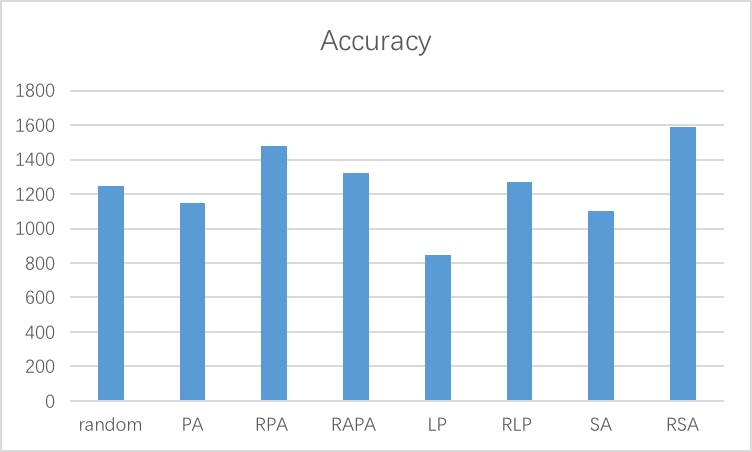
\includegraphics[trim=0 10 0 0]{road.png}}
\caption{In this experiment, we first create a California road network, the data was obtained from stanford Datasets.Intersections and endpoints are represented by nodes and the roads connecting these intersections or road endpoints are represented by undirected edges.The network contains 1,965,206	 nodes and 2,766,607 edges.Since the network is too large to process, so we need to select a part of the graph. We randomly choose a node from the network, like nodeId= 800120, then we regard the node as the center node, next we use the center node to spread out the network, just like BFS algorithm.Here in this experiment, we set the spread level equals 15, and we get the network with 223 nodes and 291 edges.}\label{BAZD}
\end{figure}

Since road network has the lowest heterogeneity among BA and USAir, the degree of the nodes in the network mainly lies in 1,2,3,4,5, so it is hard to identify the important of the edges. But from 10,000 round of comparison, our experiment still reveals the Negative Correlation effect in road network. RPA, RAPA, RLP, RSA performs better than random way, and PA, LP, SA performs badly.From the fig1, we can observe that RSA performs best, I think this may be the reason that we have fully utilize the information of one node in the situation of low heterogeneity. This phenomenon also remind us to use more similarity information to improve the performance of road recovery. 


\begin{figure}[ht]
\scalebox{0.5}[0.5]{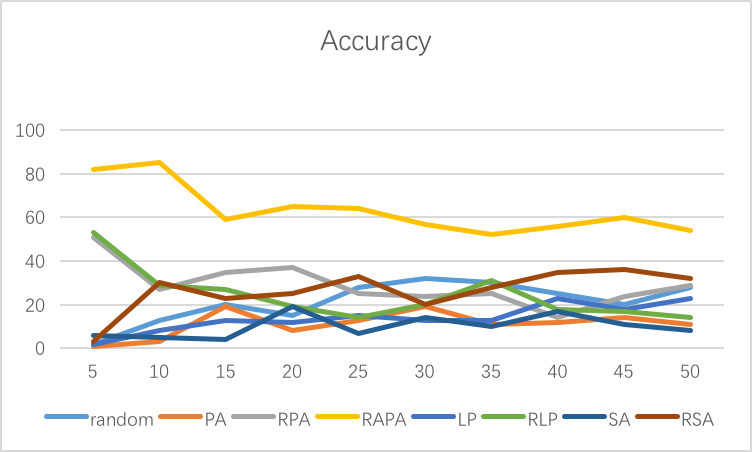
\includegraphics[trim=0 10 0 0]{baFlow.png}}
\caption{In order to verify  the robust of different methods. We have controlled the value of R. In the above experiment, we create a USAir network, it has 332 nodes and 2126 edges. We then set the ratio of destroyed edges equals to 0.05. Under different R, we got the algorithm's performance as above.}\label{BAZD}
\end{figure}


USAir is a kind of transportation system. We can see RAPA always performs best, then follows as RLP, RSA.With the increasement of R, although negative way still performs better, but the gap between positive and negative ways are becoming smaller, the reason for this phenomenon may be that at a very small value of R, the congestion  level of the roads are not serious, so the recovery of the roads can release the congestion  level a lot. But with the increase of R and congestion, the recovery of roads can't change the congestion  situation a lot, so the difference between the recovery methods isn't as big as above. Since the performance of negative ways overwhelms positive link prediction methods under different traffic flow rate, so our methods proves to be robustness. Since normal traffic system won't be too congested, so negative methods can be far more better than random recover the routes. 


\begin{table}[tbp]
\centering  % 表居中
\begin{tabular}{lcccccccccc}  % {lccc} 表示各列元素对齐方式,left-l,right-r,center-c
\hline  % \hline 在此行下面画一横线
R &5 &10 &15 &20 &25 &30 &35 &40 &45 &50\\ 
\hline  Order parameter &0.005 &0.24 &0.34 &0.46 &0.54 &0.60 &0.64 &0.68 &0.70 &0.73\\  
\hline
\end{tabular}
\caption{Correspond to Fig.2, the average order parameter in different value of R. }
\end{table}


\begin{figure}[ht]
\scalebox{0.5}[0.5]{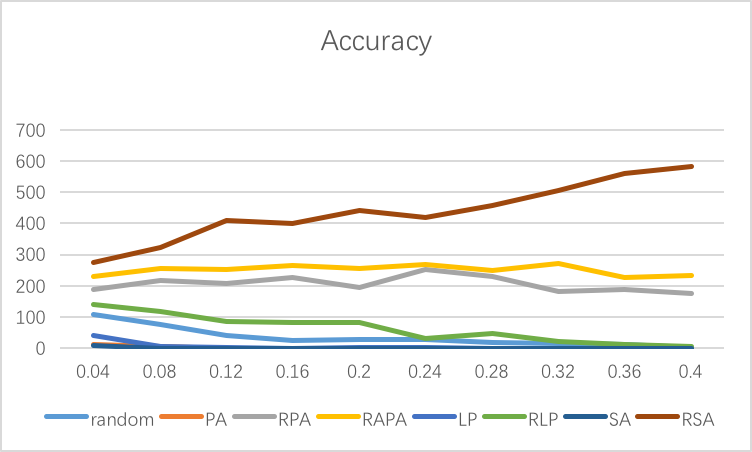
\includegraphics[trim=0 10 0 0]{fractionSize.png}}
\caption{In order to know how congestion  ratio affect the recovery of traffic. We have generate a BA network with 256 nodes and 508 edges, x-axis represent the ratio of congested route. In the above picture, 0.04 means there are int(0.04*508) edges have been congested. Y-axis represent the accurate prediction sequences in 1000 round experiment. The packages generated in one time step is 10.}\label{BAZD}
\end{figure}


A lot of traffic system can be modeled as BA network. From fig.3 we can see with the increasement of fraction ratio, negative recovery methods perform far more better than random method and positive one's. At the fraction ratio of 0.4, in 1000 round experiment, RSA method performs best in about 600 round comparison, RPA and RAPA performs about 200 round best respectively while other methods almost have no chance in the guidance of traffic recovery. I think there are two reason for the result, with the increasement of fraction ratio, the recovery sequences have  more combination so we can differentiate them more easily. Another reason is that big fraction ratio requires more time in the recovery process, in a larger period of time, we can verify our methods more easily. 


\begin{figure}[ht]
\scalebox{0.5}[0.5]{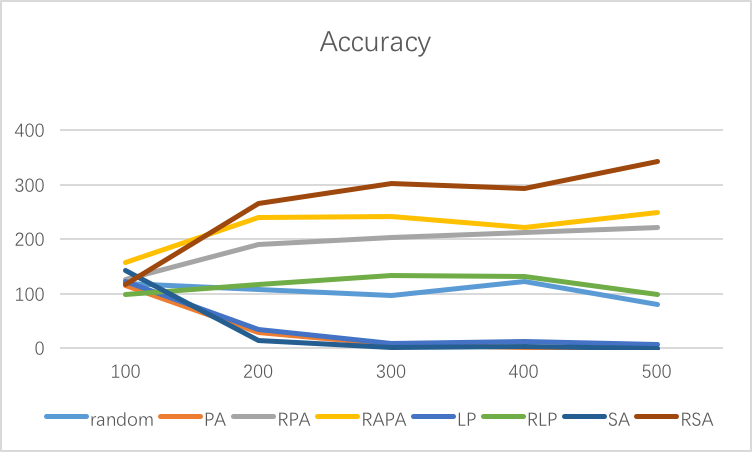
\includegraphics[trim=0 10 0 0]{baSize.png}}
\caption{To test our methods in different size of networks, we have generate five BA networks, they contain nodes with 100, 200, 300, 400, 500 respectively. The probability for each node to generate a package in one time step is 0.02 and the fraction ratio is 0.05.}\label{BAZD}
\end{figure}


In fig.4 we can see that when the network contains 100 nodes, eight methods haven't much difference in the traffic recovery, this is mainly because that at a very small network there are no big difference for each node so we can't distinguish them clearly. But when the size of the net reaches a certain scale, nodes in the network play roles quite differently, hub nodes and normal nodes can't be the same. When the size of BA network reaches 200, the difference of performance can be observed easily. With the increasement of BA size, negative recovery methods perform better than random method and positive methods. At the size of 500, positive ways almost have no chance in accurately recover the routes in a certain sequence. The reason for that negative methods in larger BA network plays better mainly because the larger BA network has larger heterogeneity, so the nodes play roles differently and we can distinguish them more easily. Normally traffic system won't be too small, they usually contain nodes over 200, so our negative ways can be of use in routes recovery especially the reverse similarity(RSA) method. 


\section*{CONCLUSION}
Traffic  problem affect the operation efficiency of the society, current study mainly focus on add new route or rebuild the network. But even the best system can't avoid congestion  entirely. Our methods mainly focus on how to recover the routes sequences in a certain order to minimize the negative impact. Inspired by link prediction methods, we have recovered the the route in three strategies. These strategies are positive ways which include PA, LP and SA; negative ways which include RPA, RAPA, RLP and RSA; random way. From our experiment we find that negative ways perform better than the random recover of routes, random way are better than positive ways which is obviously since negative ways and positive ways are reverse methods. Beside the verification of negative link prediction methods in routes recovery. We also find that larger network can improve negative link prediction methods' accuracy; Higher degree heterogeneity improves experiment accuracy also, so negative methods are effective especially for BA like topological; At a high level of congested routes like half of the routes have been broken, negative methods almost have accuracy of 100\% in the routes recovery.

Our study is tentative in using link prediction methods solving traffic problem, our result shows a tremendous potential combine link prediction methodology and real traffic problem. Since few people have doing researches in this field, so there are many shortcomings to be further optimized. In lack of real traffic flow data, so we simplified our simulation with a certain rate of packages generated in a certain time step. If possible, further studies can obtain real traffic flow and doing recovery experiment. Also weighted networks deserve to be discussed. In all, our research have found some simple ways to recover the congested ways efficiently, this may a new branch in the traffic problem.

\section*{Author contributions}
Yichao Zhang and Xing Li contribute equally.







\section*{References}
\begin{thebibliography}{00}

\bibitem{TFWN}Traffic fluctuation on weighted networks

\bibitem{PSV} R. Pastor-Satorras and A. Vespignani, “Epidemic spreading in scale-free networks,” Phys. Rev. Lett., vol. 86, pp. 3200–3203, 2001.

\bibitem{AEM} A. E. Motter and Y. C. Lai, “Cascade-based attacks on complex net- works,” Phys. Rev. E, vol. 66, no. 065102, 2002.

\bibitem{KIG} K. I. Goh, D. S. Lee, B. Kahng, and D. Kim, “Sandpile on scale-free net- works,” Phys. Rev. Lett., vol. 91, no. 148701, 2003.

\bibitem{BTS} B. Tadic ́, S. Thurner, and G. J. Rodgers, “Traffic on complex networks: Towards understanding global statistical properties from microscopic density fluctuations,” Phys. Rev. E, vol. 69, no. 036102, 2004.

\bibitem{LZYC} L. Zhao, Y. C. Lai, K. Park, and N. Ye, “Onset of traffic congestion in com- plex networks,” Phys. Rev. E, vol. 71, no. 026125, 2005.

\bibitem{HHM} H. Hong, M. Y. Choi, and B. J. Kim, “Synchronization on small-world net- works,” Phys. Rev. E, vol. 65, no. 026139, 2002.

\bibitem{RAA} R. Albert and A.-L. Barabási, “Statistical mechanics of complex net- works,” Rev. Mod. Phys., vol. 74, pp. 47–97, 2002.

\bibitem{SND} S. N. Dorogvtsev and J. F. F. Mendes, “Evolution of networks,” Adv. Phys., vol. 51, pp. 1079–1187, 2002.

\bibitem{MEJ} M. E. J. Newman, “The structure and function of complex networks,” SIAM Rev., vol. 45, pp. 167–256, 2003.

\bibitem{SBV} S. Boccaletti, V. Latora, Y. Moreno, M. Chavez, and D.-U. Hwanga, “Com- plex networks: Structure and dynamics,” Phys. Rep., vol. 424, pp. 175–308, 2006.

\bibitem{TCIC}Traffic congestion in interconnected complex networks

\bibitem{GTC}N. Biggs, E. K. Lloyd, and R. J. Wilson. Graph Theory, 1736-1936. Claren- don Press, New York, NY, USA, 1986.

\bibitem{LPU}MohammadAlHasan,VineetChaoji,SaeedSalem,andMohammedZaki. Link prediction using supervised learning. In In Proc. of SDM 06 workshop on Link Analysis, Counterterrorism and Security, 2006.

\bibitem{NPA}Ryan N. Lichtenwalter, Jake T. Lussier, and Nitesh V. Chawla. New per- spectives and methods in link prediction. In Proceedings of the 16th ACM SIGKDD International Conference on Knowledge Discovery and Data Min- ing, KDD ’10, pages 243–252, New York, NY, USA, 2010. ACM.

\bibitem{LPC}Zhen Liu, Qian-Ming Zhang, Linyuan Lü, and Tao Zhou. Link prediction in complex networks: A local naïve bayes model. EPL (Europhysics Letters), 96(4):48007, 2011.

\bibitem{WWC}Andrew Chen-Brian Tran Ole J. Mengshoel, Raj Desai. Will we connect again? machine learning for link prediction in mobile social networks. 2013.

\bibitem{SRM}Kai Yu, Wei Chu, Shipeng Yu, Volker Tresp, and Zhao Xu. Stochastic
relational models for discriminative link prediction. In Advances in Neural Information Processing Systems, pages 333–340. MIT Press, 2007.

\bibitem{GME}Edward J Taaffe,Howard L Gauthier,Morton E.0’KeHy.
Geography of Transportation(2nd).Prentice Hall,1996.

\bibitem{GOT}odrigue J P et a1.ne Geography of Transport Systems,
Hofstra Univemity.Department of Economics\& Geogra

\bibitem{UTN}Sheffi,Yose[Urban Transportation Networks:Equilibrium Analysis with Mathematical Programming Methods.Prentice-Hall,Inc,1 985.

\bibitem{NHS}A. Clauset, C. Moore, M. E. J. Newman, Hierarchical structure and the prediction of missing links in networks, Nature 453 (2008) 98.

\bibitem{TOM}S. Redner, Teasing out the missing links, Nature 453 (2008) 47.

\bibitem{SPR}J. O’Madadhain, J. Hutchins, P. Smyth, Prediction and ranking algorithms for event-based network data, In Proceedings of SIGKDD 2005, ACM Press, New York, 2005, p. 23.

\bibitem{TZ}T. Zhou, J. Ren, M. Medo, Y.-C. Zhang, Bipartite network projection and personal recommendation, Phys. Rev.E 76 (2007) 046115.

\bibitem{SAD}T. Zhou, Z. Kuscsik, J.-G. Liu, M. Medo, J. R. Wakeling, Y.-C. Zhang, Solving the apparent diversity-accuracy dilemma of recommender systems, Proc. Natl. Acad. Sci. U.S.A. 107 (2010) 4511.

\bibitem{CAA}W. Zeng, M.-S. Shang, Q.-M. Zhang, L. Lu ̈, T. Zhou, Can dissimilar users contribute to accuracy and diversity of personalized recommendation, Int. J. Mod. Phys. C (to be published).

\bibitem{SV}Lü, Linyuan, and T. Zhou. "Link prediction in complex networks: A survey." Physica A Statistical Mechanics \& Its Applications 390.6(2011):1150-1170.


\bibitem{WG}Xie Y B, Zhou T, Wang B H. Scale-free networks without growth[J]. Physica A Statistical Mechanics \& Its Applications, 2008, 387(7):1683-1688.

\bibitem{LI}Zhou T, Lü L, Zhang Y C. Predicting missing links via local information[J]. \bibitem{AC}The European Physical Journal B, 2009, 71(4):623-630.
Ackland R, Ackland R. Mapping the U.S. Political Blogosphere: Are Conservative Bloggers More Prominent?[C]// 2005.

\bibitem{BA}A.-L. Barabási and R. Albert, Science 286, 509 (1999).

\bibitem{PML}Zhou T, Lü L, Zhang Y C. Predicting missing links via local information[J]. The European Physical Journal B, 2009, 71(4):623-630.
71(4):623–630. 

\bibitem{KD}Zhang Y, Aziz-Alaoui M A, Bertelle C, et al. Knowledge Diffusion in Complex Networks[C]// IEEE, Intl Conf on Ubiquitous Intelligence and Computing and 2015 IEEE, Intl Conf on Autonomic and Trusted Computing and 2015 IEEE, Intl Conf on Scalable Computing and Communications and ITS Associated Workshops. 2015.

\bibitem{SW}Watts DJ, Strogatz SH. Collectivedynamics of ’small-world’ networks[C]// Nature. 1998:440-442.

\bibitem{BVL}S. Boccaletti, V. Latora, Y. Moreno, M. Chavez, and D.-U.Hwang, Phys. Rep. 424, 175 (2006).

\bibitem{MEN}S. N. Dorogovtsev, J. F. F. Mendes. Evolution of networks[M]// Evolution of networks :. Oxford University Press, 2003:1842-1845.


\bibitem{LCS}[1] L. Cui, S. Kumara, and R. Albert, IEEE Circuits and Systems Magazine 10, 10 (2010).
\bibitem{LZY}[2] L. Zhao, Y.-C. Lai, K. Park, and N. Ye, Phys. Rev. E 71, 026125 (2005).
\bibitem{AAA}[3] A. Arenas, A. D ́ıaz-Guilera, and R. Guimer`a, Phys. Rev. Lett. 86, 3196 (2001).
\bibitem{DDL}[4] D. De Martino, L. Dall’Asta, G. Bianconi, and M. Mar- sili, Physical Review E 79, 015101 (2009).
\bibitem{JWC}[5] J. Wu, C. Tse, F. C. Lau, and I. W. Ho, IEEE Trans. Circuits Syst. I, Reg. Papers 60, 3303 (2013).
\bibitem{SBV}[6] S. Boccaletti, V. Latora, Y. Moreno, M. Chavez, and D.- U. Hwang, Phys. Rep. 424, 175 (2006).
\bibitem{RGA}[7] R. Guimer`a, A. Arenas, A. D ́ıaz-Guilera, and F. Giralt, Phys. Rev. E 66, 026704 (2002).

\bibitem{SCW}[9] S. Chen, W. Huang, C. Cattani, and G. Altieri, Mathe- matical Problems in Engineering 2012, 732698 (2012).
\bibitem{GYT}[10] G. Yan, T. Zhou, B. Hu, Z.-Q. Fu, and B.-H. Wang, Phys. Rev. E 73, 046108 (2006).
\bibitem{BDY}[11] B. Danila, Y. Yu, J. A. Marsh, and K. E. Bassler, Phys. Rev. E 74, 046106 (2006).
\bibitem{XLM}[12] X. Ling, M.-B. Hu, R. Jiang, and Q.-S. Wu, Phys. Rev. E 81, 016113 (2010).
\bibitem{FTY}[13] F. Tan and Y. Xia, Physica A 392, 4146 (2013).
\bibitem{YXD}[14] Y. Xia and D. Hill, EPL 89, 58004 (2010).
\bibitem{XLMD}[15] X. Ling, M.-B. Hu, J.-C. Long, J.-X. Ding, and Q. Shi,
Chin. Phys. B 22, 018904 (2013).
\bibitem{GQZ}[16] G.-Q. Zhang, S. Zhou, D. Wang, G. Yan, and G.-Q.
Zhang, Physica A 390, 387 (2011).
\bibitem{ZTKE}[137] Z. Toroczkai, K.E. Bassler, Nature 428 (2004) 716.
\bibitem{ZTBE}[138] Z. Toroczkai, B. Kozma, K.E. Bassler, N.W. Hengartner, G. Korniss, preprint cond-mat/0408262.

\end{thebibliography}



\end{document}
